\documentclass[a4paper, 12pt]{article}
\usepackage[utf8x]{inputenc}
\usepackage[english, russian]{babel}
\usepackage[left=25mm, top=25mm, right=25mm, bottom=25mm]{geometry}
\usepackage{cmap}
\usepackage{indentfirst}
\usepackage{tikz}
\usepackage{float}
\usepackage{amsmath, amsfonts, amssymb}
\usepackage{graphicx}
\usepackage{hyperref}
\usepackage{listings}
\usepackage{caption}
\usepackage{subcaption}
\usepackage{xcolor}
\usepackage{etoolbox}
\usepackage{titlesec}
\usepackage{array}
\pagestyle{plain}
\patchcmd{\tableofcontents}{\contentsname}{\centering\contentsname}{}{}
\titleformat{\section}[block]{\normalfont\large\bfseries\centering}{}{0pt}{}
\titleformat{\subsection}[block]{\normalfont\normalsize\bfseries\centering}{}{0pt}{}
\allowdisplaybreaks
\graphicspath{{src/images/}}
\usetikzlibrary{patterns}
\definecolor{LightGray}{gray}{0.95}
\definecolor{LightGray2}{gray}{0.7}
\hypersetup{
    colorlinks=true,
    linkcolor=blue,
    filecolor=magenta,
    urlcolor=cyan,
    pdftitle={contents setup},
    pdfpagemode=FullScreen,
}


\begin{document}
    \begin{titlepage}

        \begin{center}
        Федеральное государственное автономное образовательное учреждение высшего образования
        «Национальный Исследовательский Университет ИТМО»
        \vfill
        
        
\includegraphics[width=0.3\textwidth]{itmo.png} % requires /src/images/itmo.png

        {\large\bf ЛАБОРАТОРНАЯ РАБОТА №2}\\
        {\large\bf ПРЕДМЕТ «ЭЛЕКТРОННЫЕ УСТРОЙСТВА СИСТЕМ УПРАВЛЕНИЯ»}\\
        {\large\bf ТЕМА «СТАБИЛИЗАТОРЫ НАПРЯЖЕНИЯ»}\\
        Вариант №5
        \vfill

        \begin{flushright}
            \begin{minipage}{.45\textwidth}
            {
                \hbox{Преподаватель:}
                \hbox{Жданов В. А.}
                \hbox{}
                \hbox{Выполнил:}
                \hbox{Румянцев А. А.}
                \hbox{}
                \hbox{Факультет: СУиР}
                \hbox{Группа: R3341}
                \hbox{Поток: ЭлУСУ R22 бак 1.2}
            }
            \end{minipage}
        \end{flushright}
        \vfill
  
        Санкт-Петербург\\
        2025
        \end{center}
    \end{titlepage}
    
    \tableofcontents

    \newpage
    \section{Цель работы}
    Цель работы -- исследование и сравнение характеристик различных схемных решений
    стабилизаторов на дискретных элементах и стабилизатора в интегральном исполнении.


    \section{Исходные данные}
    В таблице ниже представлены исходные данные для варианта №5
    \begin{center}
        \begin{tabular}{ | m{4em} | m{2em}| } 
        \hline
        $U_{\text{вых.}}$, В& $8$\\ 
        \hline
        $R_{\text{н.}}$, Ом& $3500$\\ 
        \hline
        $U_{\text{вх.}}$, В& $16$\\ 
        \hline
        \end{tabular}
    \end{center}


    \section{Исследование параметрического стабилизатора}
    \subsection{Выбор стабилитрона}
    Выходное напряжение (напряжение стабилизации) составляет 8 В, тогда возьмем стабилитрон типа EDZV8.2B $\Rightarrow U_{\text{ст.}}=8.2$ В.
    При подаче 8.2 В он начнет проводить ток (при $<8.2$ В ничего не будет делать, при $>8.2$ В <<сбросит>>
    лишнее напряжение через себя, удерживая на нагрузке примерно 8.2 В; теперь $U_{\text{вых.}}=8.2$ В). Этот стабилитрон имеет рассеиваемую
    мощность $P_\text{ст.}=0.15$ Вт, дифференциальное сопротивление $r_{\text{ст.}}=30$ Ом
    
    
    \subsection{Расчет схемы}
    Рассчитаем максимальный ток, текущий
    через стабилитрон
    $$
    I_{\text{ст. макс.}}=\dfrac{P_{\text{ст.}}}{U_{\text{ст.}}}=\dfrac{0.15}{8.2}=0.0182926829\text{ А}
    $$
    Рассчитаем ток нагрузки
    $$
    I_{\text{н.}}=I_{\text{ст.}}=\dfrac{U_{\text{вых}}}{R_{\text{н.}}}=\dfrac{8.2}{3500}=0.0023428571\text{ А}
    $$
    Рассчитаем номинальное значение тока на стабилитроне
    $$
    I_{\text{ст. ном.}}=\dfrac{I_{\text{ст. макс.}}-I_{\text{ст.}}}{2}=\dfrac{0.018-0.002}{2}=0.0079749129\text{ А}
    $$
    Определим балластное сопротивление резистора
    $$
    R_{\text{б.}}=\dfrac{U_{\text{вх.}}-U_{\text{вых.}}}{I_{\text{ст. ном.}}+I_{\text{н.}}}=\dfrac{16-8.2}{0.008+0.002}=755.9773090503\text{ Ом}
    $$


    \subsection{Коэффициент стабилизации}
    Определим коэффициент стабилизации
    $$
    k_{\text{ст.}}=\left( 1-\dfrac{R_{\text{б.}}\left( I_\text{ст. ном.}+I_{\text{н.}} \right)}{U_{\text{вх.}}} \right)\cdot\dfrac{R_{\text{б.}}+r_{\text{ст.}}}{r_{\text{ст.}}},
    $$
    $$
    k_{\text{ст.}}=\left( 1-\dfrac{755.977\left( 0.008+0.002 \right)}{16} \right)\cdot\dfrac{755.977+30}{30}=13.4271123629;
    $$
    Посчитаем оценку $k_{\text{ст.}}$ (приближенно коэффициент стабилизации)
    $$
    \hat{k}_{\text{ст.}}=\dfrac{R_{\text{б.}}U_{\text{вых.}}}{r_{\text{ст.}}U_{\text{вх.}}}=12.9146123629
    $$


    \subsection{Коэффициент полезного действия}
    Определим коэффициент полезного действия
    $$
    \eta=\dfrac{I_\text{ст. ном.}U_{\text{ст.}}}{U_{\text{вх.}}\left( I_{\text{ст. ном.}}+I_{\text{н.}} \right)}=\dfrac{0.008\cdot8.2}{16\left( 0.008+0.002 \right)}=0.3961265720\approx40\%
    $$


    \subsection{Схема параметрического стабилизатора}
    Соберем схему параметрического стабилизатора с учетом наших расчетов.
    Конденсатор в расчетах не участвовал (со временем перестанет проводить ток)
    -- он нужен для сглаживания пульсаций (фильтр шумов)
    \begin{figure}[H]
        \centering
        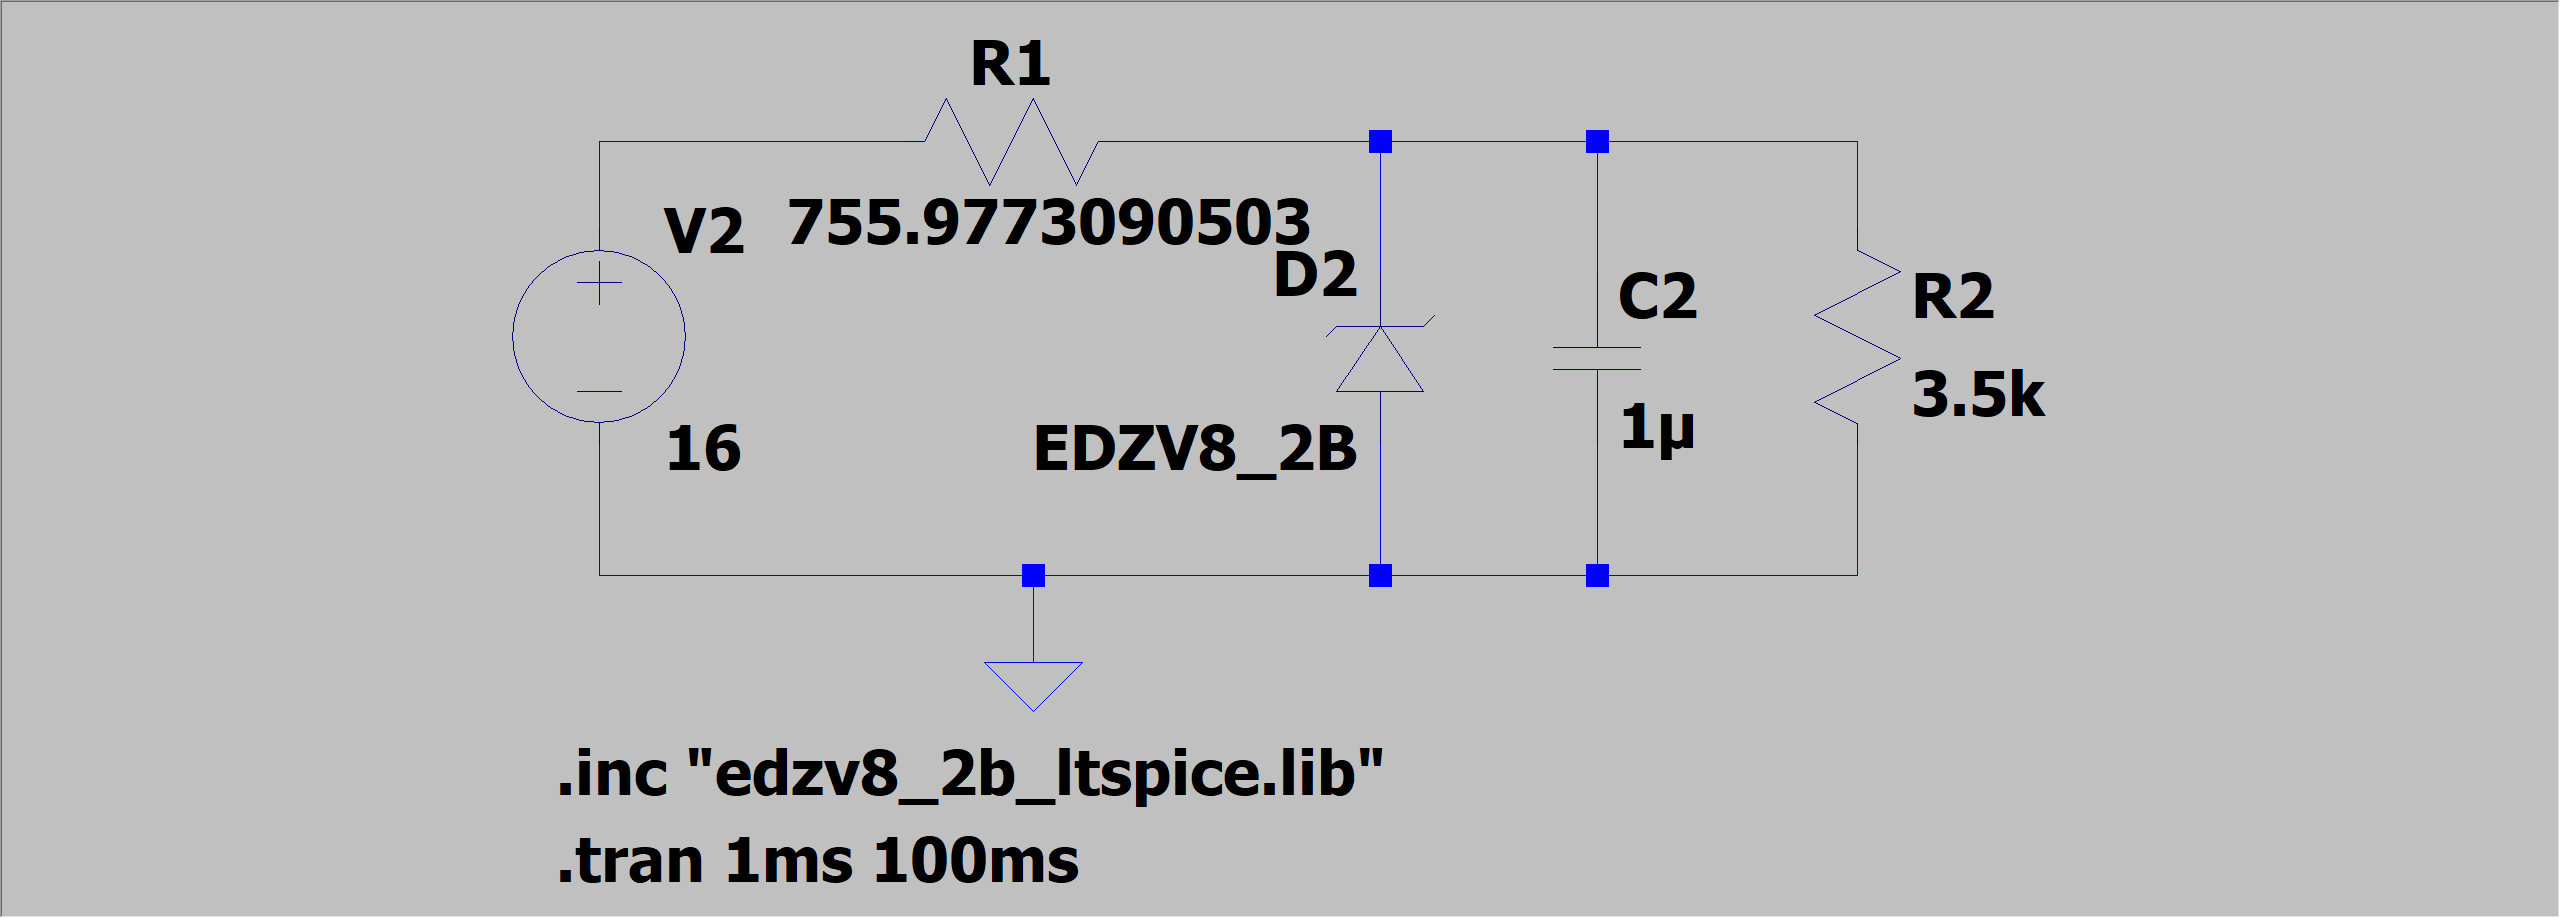
\includegraphics[scale=0.22]{scheme1.png}
        \captionsetup{skip=0pt}
        \caption{Схема параметрического стабилизатора}
        \label{fig:scheme1}
    \end{figure}
\end{document}